\documentclass{tufte-book}
\usepackage{graphicx}
\usepackage{lipsum}
\setkeys{Gin}{width=\linewidth,totalheight=\textheight,keepaspectratio}
% Prints a trailing space in a smart way.
\usepackage{xspace}


\usepackage{hyperref}
\usepackage{amsmath}

\newcommand{\tthdump}[1]{#1}
\usepackage{makeidx}
\makeindex

\title{My title}

\usepackage{Sweave}
\begin{document}
\setkeys{Gin}{width=1.1\marginparwidth} %% Sweave

 \section{Where I get both funky and fresh}
\begin{Schunk}
\begin{Sinput}
>   set.seed(12)
>   t <- rnorm(100)
\end{Sinput}
\end{Schunk}
and an example plot
\begin{center}
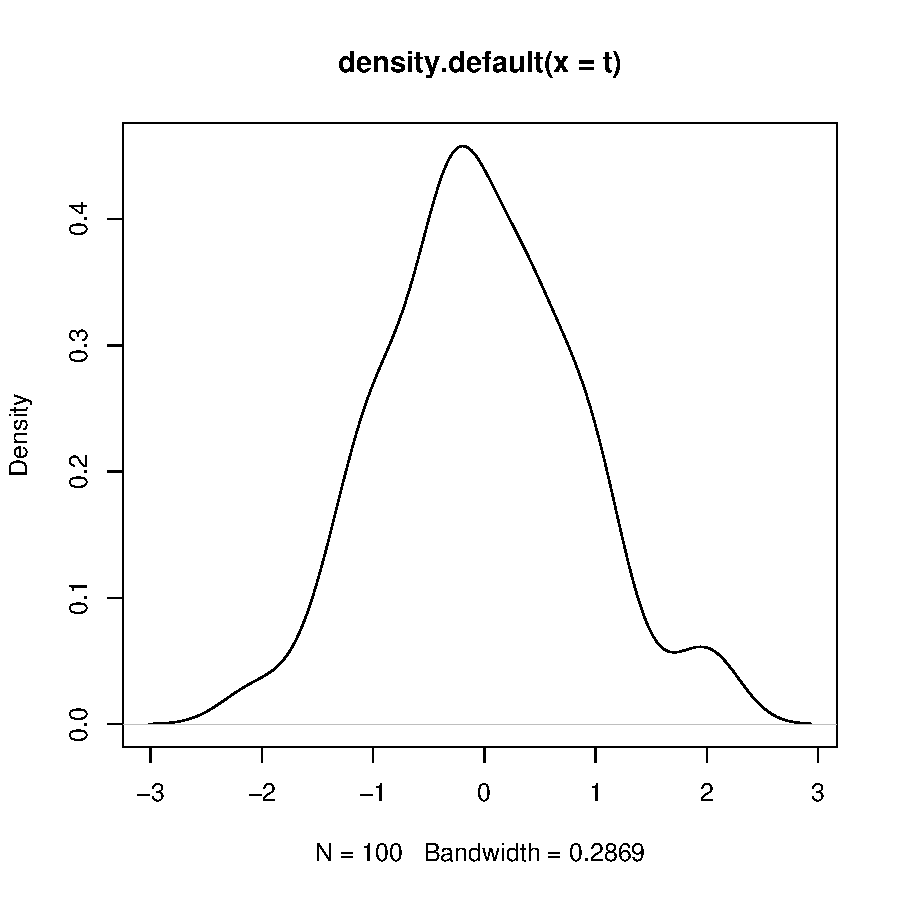
\includegraphics{SweaveExample-002}
\end{center}

%% a margin figure
\begin{marginfigure}
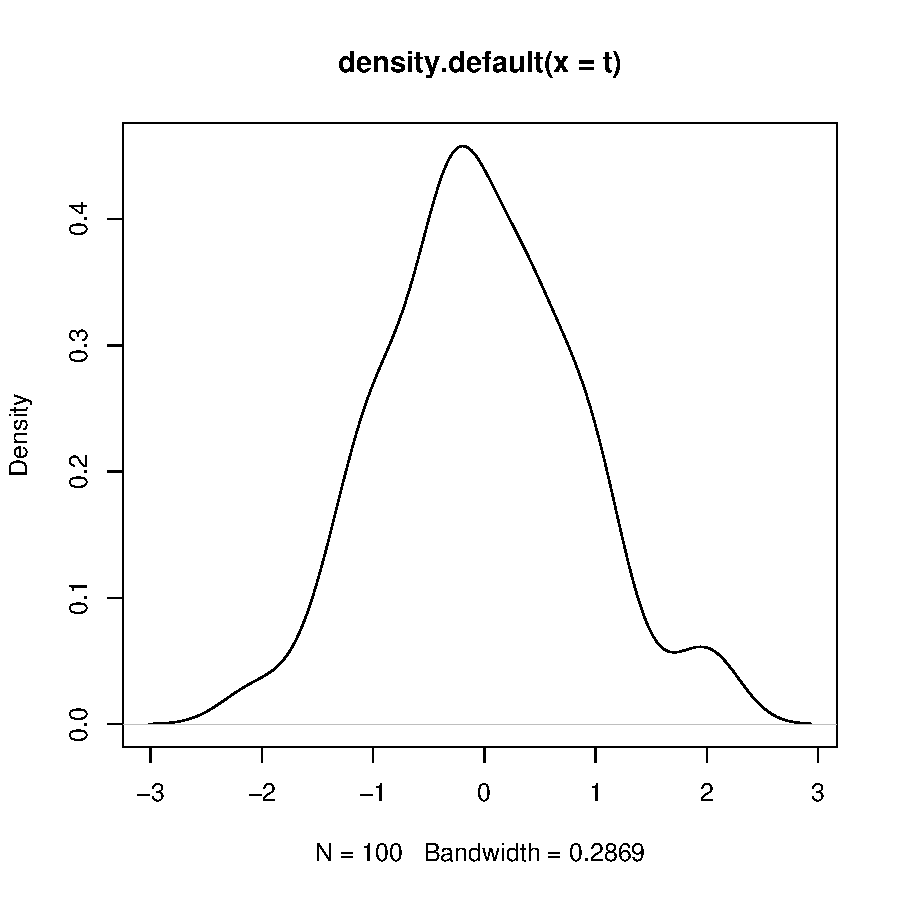
\includegraphics{SweaveExample-004}
\end{marginfigure}

This is a very simple example of how we might get started with Sweave. You know what comes next, right? That's right... Lorem Ipsum, ladies! 
\lipsum

\end{document}
